\section{Results \& discussion}
\label{sec:resul}

For a better understanding of the results of this work it is important to note how PM10 concentrations affect air quality.
In Table \ref{table:pm10-classification} one can see the official classification of the PM10 concentration values \cite{QualAr}.

\definecolor{springgreen}{rgb}{0.0, 0.65, 0.31}
\definecolor{carrotorange}{rgb}{0.93, 0.57, 0.13}
\definecolor{electricgreen}{rgb}{0.0, 1.0, 0.0}
\definecolor{bostonuniversityred}{rgb}{0.8, 0.0, 0.0}
\begin{table}[ht]
\centering
\footnotesize
\caption{Classification of PM10 concentration.}
\label{table:pm10-classification}
\begin{tabular}[t]{>{\centering}p{0.2\linewidth}>{\centering\arraybackslash}p{0.4\linewidth}}
\toprule
Classification&PM10 concentration interval ($\mu g/m^3$)\\
\midrule
\cellcolor{electricgreen}Very Good& 0 - 20\\
\cellcolor{springgreen}Good& 21 - 35\\
\cellcolor{yellow}Medium& 36 - 50\\
\cellcolor{carrotorange}Weak& 51 - 100\\
\cellcolor{red}Bad& 101 - 1200\\
\bottomrule
\end{tabular}
\end{table}%

It can be observed that the smallest classification interval corresponds to 14 $\mu g/m^3$, for both Good and Medium intervals.

\subsection{NB-IoT PM10 Monitoring System}

In Table \ref{table:measurement-period} are presented the weeks during which the developed system was placed in a CCDR-LVT station. 

\definecolor{springgreen}{rgb}{0.0, 0.65, 0.31}
\definecolor{bostonuniversityred}{rgb}{0.8, 0.0, 0.0}
\renewcommand\arraystretch{1.5}
\renewcommand{\tabcolsep}{3pt}
\begin{table}[ht]
\centering
\footnotesize
\caption{Coverage during the developed system placement.}
\label{table:measurement-period}
\begin{tabular}[t]{l>{\centering}p{0.057\linewidth}>{\centering}p{0.057\linewidth}>{\centering}p{0.057\linewidth}>{\centering}p{0.057\linewidth}>{\centering}p{0.057\linewidth}>{\centering}p{0.057\linewidth}>{\centering}p{0.057\linewidth}>{\centering}p{0.057\linewidth}>{\centering}p{0.057\linewidth}>{\centering\arraybackslash}p{0.057\linewidth}}
\toprule
&\multicolumn{2}{c}{July}&\multicolumn{4}{c}{August}&\multicolumn{4}{c}{September}\\
\midrule
{}Week&3&4&1&2&3&4&1&2&3&4\\
\midrule
AVL&\cellcolor{bostonuniversityred}&\cellcolor{bostonuniversityred}&&&&&&&\cellcolor{springgreen}&\cellcolor{springgreen}\\
ENC&&&\cellcolor{bostonuniversityred}&\cellcolor{bostonuniversityred}&\cellcolor{bostonuniversityred}&\cellcolor{bostonuniversityred}&\cellcolor{bostonuniversityred}&\cellcolor{bostonuniversityred}&&\\
\bottomrule
\end{tabular}
\end{table}

Colored cells represent the location where the developed sensor was placed during each week. In weeks colored in green, consistent measures were taken since there was NB-IoT coverage. In red colored weeks, it was impossible to get consistent coverage and consequently no measures were obtained.

In Figure \ref{fig:system-calibration}, simultaneous measures of both sensors during the placement period can be observed, along with RH measures obtained for Lisbon during the same period. The absolute error between the measures of the different sensors is 14.40 $\mu g/m^3$.

The PMS5003 sensor often obtained lower measures. However, sometimes it peaked, surpassing the reference sensor, the Environnement S.A. Model MP101M measures. This only happened for high values of RH. When the RH decreases, there is often less error between sensors.
\setlength{\abovecaptionskip}{0pt plus 0pt minus 3pt}
\begin{figure*}[ht]
\centering
\footnotesize
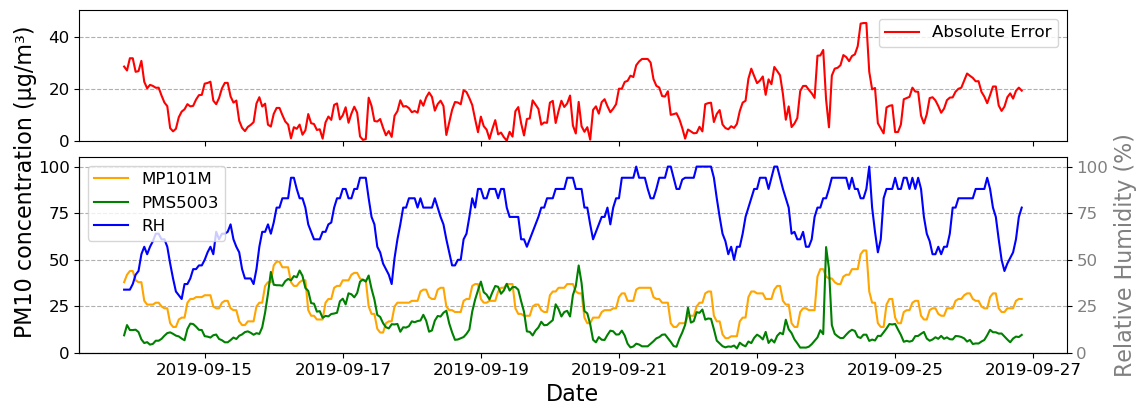
\includegraphics[width=0.9\textwidth]{./Images/calibration-thin-article.png}
\caption{PM10 concentrations reported by the sensors and simultaneous RH values.}
\label{fig:system-calibration}
\end{figure*}

The scatter diagram in Figure \ref{fig:scatter-measurements} shows that the developed system measured values are predominantly lower than the reference readings.

\setlength{\abovecaptionskip}{10pt plus 0pt minus 0pt}
\begin{figure}[ht]
\centering
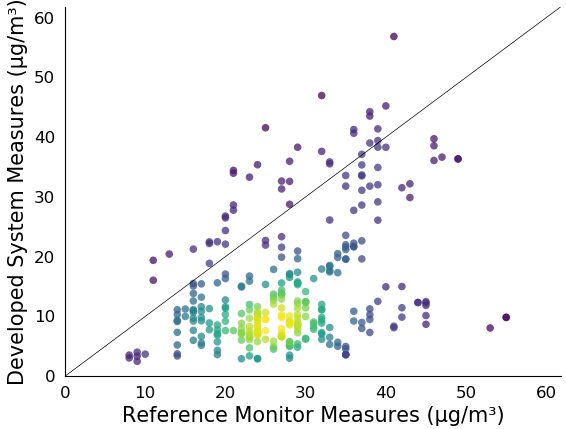
\includegraphics[width=0.45\textwidth]{./Images/scatter-measurements.png}
\caption{Scatter diagram between the developed system and the reference monitor measures.}
\label{fig:scatter-measurements}
\end{figure}

In the comparison of time series data, it is important to assess not only the error statistics between datasets, but also its linearity and correlation. 

The Pearson coefficient was calculated for every full day of the time series data, during the developed sensor placement. The coefficient obtained for the whole period was 0.39, with several days presenting negative correlation coefficients between measures.

%\begin{table*}[ht]
%\footnotesize
%\centering
%\caption{Pearson coefficients calculated for the %full days of sensor positioning.}
%\label{table:pearson-coefs-sensor}
%\begin{tabular}[t]{>{\centering}p{0.06\linewidth%}>{\centering}p{0.06\linewidth}>{\centering\arra%ybackslash}>{\centering}p{0.06\linewidth}>{\cent%ering}p{0.06\linewidth}>{\centering}p{0.06\linew%idth}>{\centering}p{0.06\linewidth}>{\centering}%p{0.06\linewidth}>{\centering}p{0.06\linewidth}>%{\centering}p{0.06\linewidth}>{\centering}p{0.06%\linewidth}>{\centering}p{0.06\linewidth}>{\cent%ering}>{\centering}p{0.06\linewidth}>{\centering%\arraybackslash}p{0.1\linewidth}}
%\toprule
%\multicolumn{12}{c}{Day of %placement}&\multirow{2}{*}{Overall}\\\cline{1-12%}
%1&2&3&4&5&6&7&8&9&10&11&12&\\
%\midrule
%0.22&0.57&0.68&0.60&0.75&0.62&0.59&-0.23&0.57  %&0.34&0.01&-0.37&0.39\\
%\bottomrule
%\end{tabular}
%\end{table*}%

\subsection{SIMs Testing}

In this section, every SIM performance test result is presented.

Through the cross validation approach application in the dataset, the IDW power function was tested with values between 0 and 5, and the value with the best error statistics was \textit{p} = 0. 

The same approach was applied in the parameter assessment of the remaining algorithms. In OK, the variogram is the main user-defined parameter. Several pre-defined variograms were tested, and in the obtained results the linear model had the lowest overall MAE and RMSE values.

In what regards FBN interpolation, both testing and training epochs, network size, number of samples and granularity of the memories of each consequent neuron were tested. The chosen parameters were 30, 30, 75, 9 and 3, respectively.

\subsubsection{SIMs Comparison}

Results regarding MAE and RMSE performance are presented in Table \ref{table:sim-comparison}, for each algorithm and each target station, for a total of 43 956 inferences.

\begin{table}[H]
\centering
\footnotesize
\caption{Model comparison results.}
\label{table:sim-comparison}
\begin{tabular}[t]{l>{\centering}p{0.075\linewidth}>{\centering}p{0.088\linewidth}>{\centering}p{0.08\linewidth}>{\centering}p{0.088\linewidth}>{\centering}p{0.08\linewidth}>{\centering}p{0.088\linewidth}>{\centering}p{0.08\linewidth}>{\centering\arraybackslash}p{0.088\linewidth}}
\toprule
&\multicolumn{2}{c}{ENC}&\multicolumn{2}{c}{ODI}&\multicolumn{2}{c}{REB}&\multicolumn{2}{c}{SCB}\\
\midrule
{} &MAE&RMSE&MAE&RMSE&MAE&RMSE&MAE&RMSE\\
\midrule
IDW&4.65&6.52&4.89&6.48&5.46&6.97&11.52&15.31\\
OK&4.67&6.52&4.89&6.49&5.55&7.06&11.41&15.18\\
FBN&5.82&7.62&6.36&8.41&7.55&9.62&11.08&14.75\\
Linear&5.90&7.74&6.59&9.46&10.11&13.11&11.04&14.51\\
NearestN&11.20&14.63&7.35&9.82&12.58&16.36&13.45&17.22\\
\bottomrule
\end{tabular}
\end{table}

The algorithms with overall lower MAE and RMSE results were IDW and OK. NN had the worse results, followed by LI. Histograms resulting from the IDW, OK and FBN execution can be observed in Figure \ref{fig:performance-histograms}.

\begin{figure}[ht]
\centering
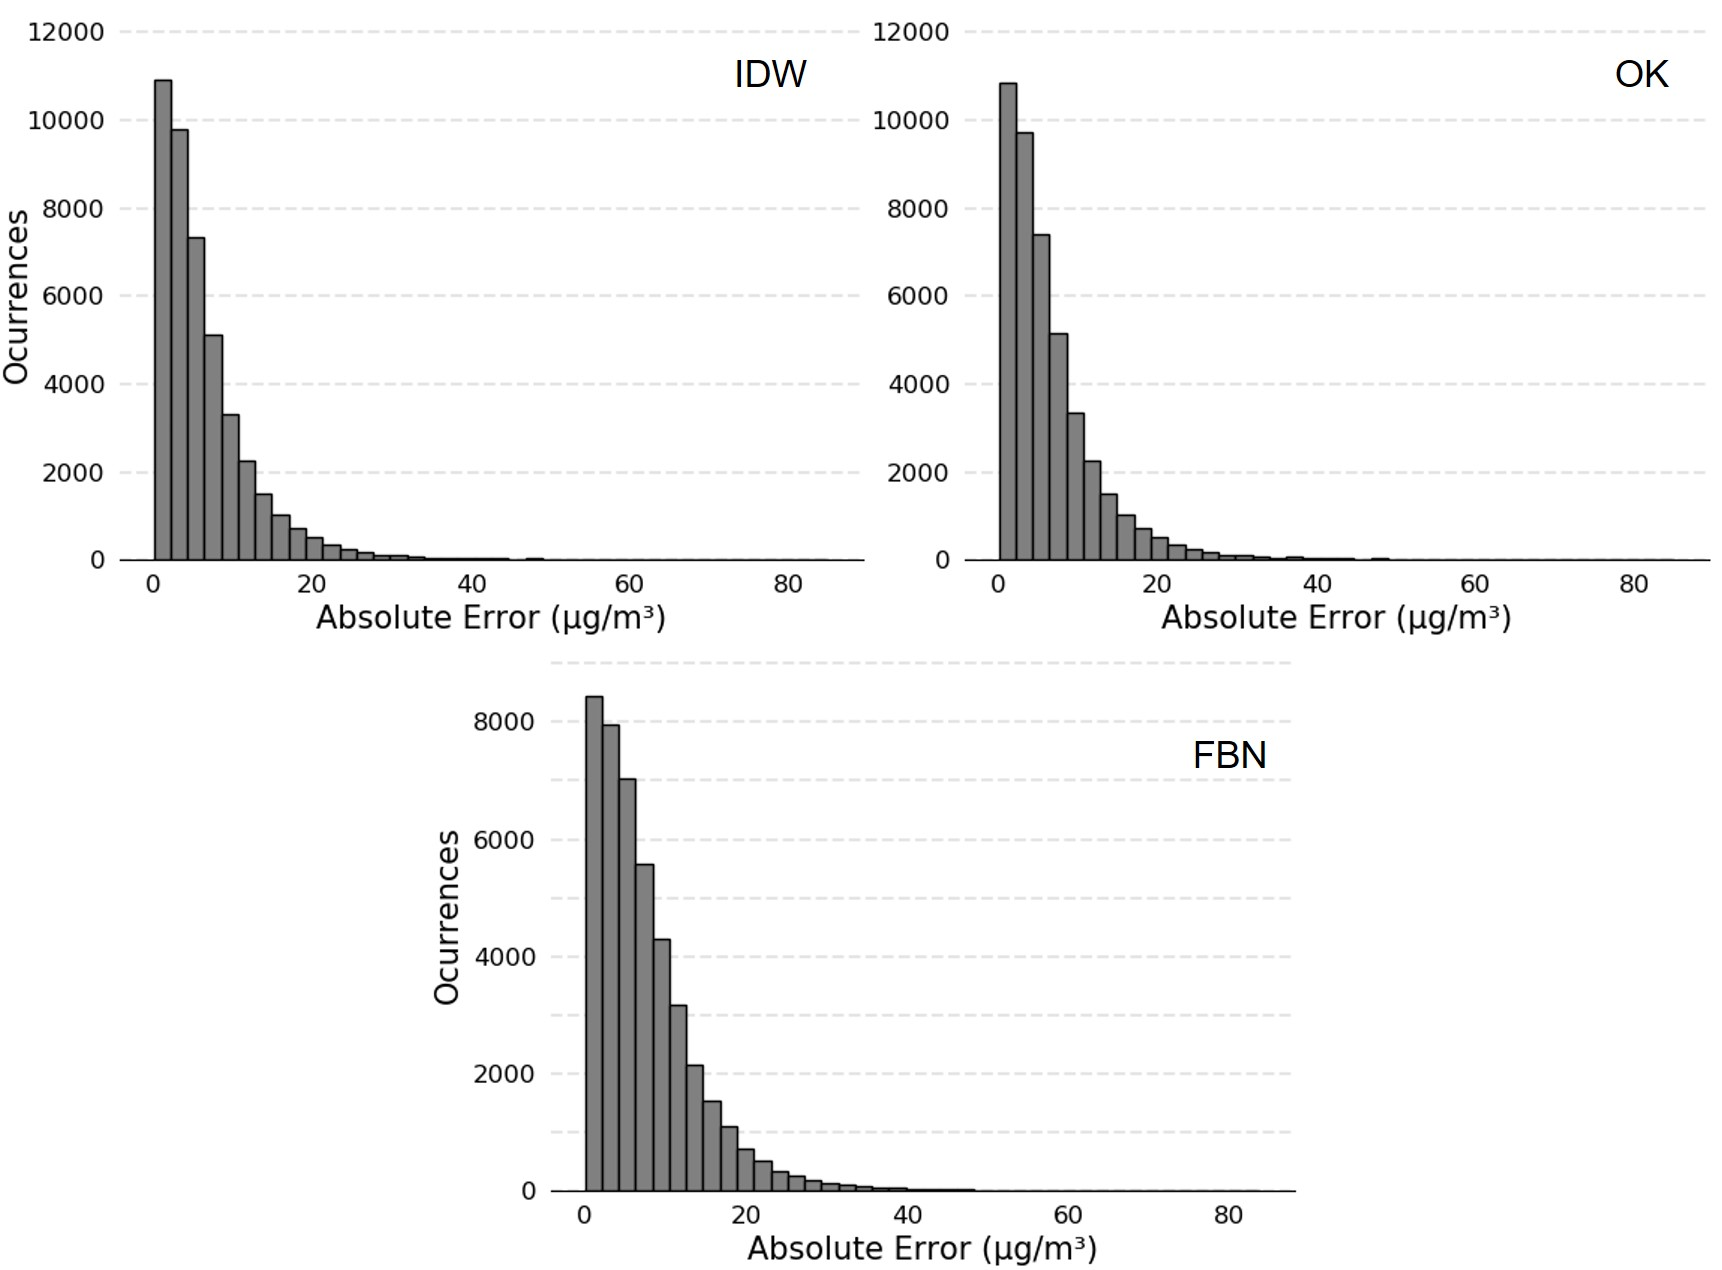
\includegraphics[width=0.49\textwidth]{./Images/performance-histograms.jpg}
\caption{Histograms obtained from 43 956 inferences for IDW, OK and FBN.}
\label{fig:performance-histograms}
\end{figure}

It should additionally be noted that, for all the inferences done simultaneously, FBNs execution times were around 9 hours, while remaining algorithms only took approximately 5 minutes.

\subsection{Online Data Visualization Web Application}

The resulting PM10 visualization application has a resolution of 100 meters, both in color and in height of the pollution surface. It provides the possibility to hover over the grid to consult estimated PM10 concentration values in any location inside the outline defined by the CCDR-LVT monitoring network stations.

The application design is focused in the user experience, and allows the user to zoom in and out, and change both pitch and bearing of the map. The final result of the developed web application is presented in Figure \ref{fig:developed-visualization}.

\begin{figure}[ht]
\centering
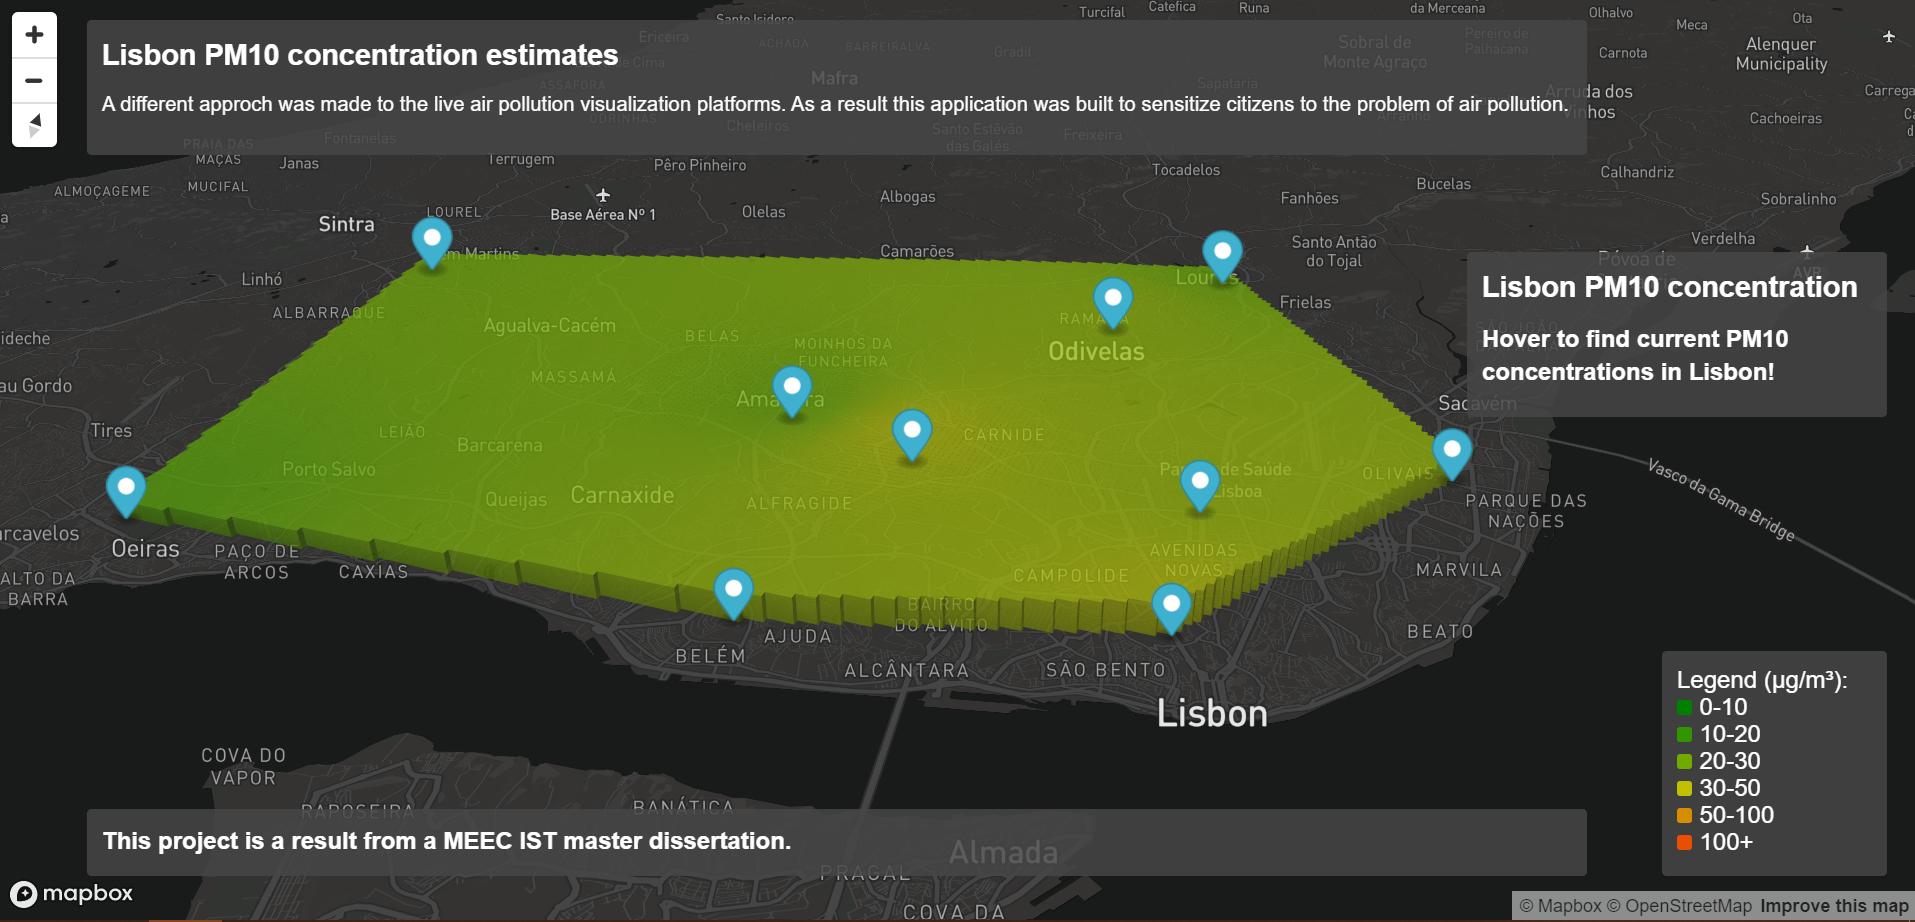
\includegraphics[width=0.47\textwidth]{./Images/developed-visualization.PNG}
\caption{Developed Web Application final result.}
\label{fig:developed-visualization}
\end{figure}

\subsection{Discussion}

%Results obtained and presented in this chapter are discussed in this section regarding every stage of this work.

\subsubsection{Developed PM10 Monitoring System}

Regarding the NB-IoT coverage in Portugal, from both MEO and NOS, namely in the capital Lisbon, it was observed that it was not good enough for professional applications at the time of this work. During the 10 weeks of testing in different locations in the city of Lisbon, there were only 2 weeks when it was possible to get consistent coverage. According to the literature \cite{Lauridsen2017}, NB-IoT has one of the widest coverage between IoT technologies. This was not observed in this work. Results demonstrated that the developed sensor, at the time of this work, from the network coverage perspective, can not be employed neither integrate current official monitoring networks.

Before assessing measurement performance, it is important to note that the obtained data only corresponds to a small sample size in comparison to what was expected.

% observations + error statistics

As mentioned, during the sensor placement and comparison period, the PMS5003 sensor often obtained lower measures (Figure \ref{fig:scatter-measurements}). However, sometimes it peaked, surpassing the MP101M measures. This only happened for high values of RH. It could additionally be observed, in Figure \ref{fig:system-calibration}, that when the RH is decreasing, there is often less error observed between the sensors.

The average absolute error between the measures of the different sensors (14.40 $\mu g/m^3$) is slightly above the smallest scale division of the classification in Table \ref{table:pm10-classification}. The daily pearson correlation coefficients showed inconsistency in the linearity between sensor readings.

It was summer season during this experiment, and the only rain occurrences during the placement periods happened in the day 21 of September. It was the day with the second highest absolute error between readings and PMS5003 measured values were lower than average in comparison to the reference sensor.

% humidity
In a study by Zheng et al., in 2018, a similar sensor model (PMS3003) was extensively tested and it was observed that while temperature took a negligible part in the difference observed between sensors, RH had a much more considerable influence \cite{Zheng2018}. 

The registered high humidity intervals correspond to night and dawn periods. 
Similar to what happened in a study by Jayaratne et al., in 2018, in these periods, measures are often higher than in the rest of the time.

In the same study, it was stated that above 75\% RH, marked effects are seen in low-cost sensors due to air particle size growth by deliquescence, specially if these do not have drying facilities at the sample inlets \cite{Jayaratne2018}. However, in this work, the only observed effects were the readings increase, which was also reported by the MP101M, and the mentioned undervalued PMS5003 measurements during the rain periods.

% car traffic
No substantial difference was observed between week and weekend days, despite the average PM10 concentration being slightly lower in both sensors.

During the day, MP101M readings are mostly higher than the taken by PMS5003.
According to Jayaratne et al., in the same study \cite{Jayaratne2018}, this may happen because the size of traffic particles are below the minimum detectable size limit of the PMS sensors. It is documented that the diameter of particles emitted by vehicles can be mostly below 300 nm \cite{Li2018}.

% conclusion on placement in official networks
Due to the numerous disadvantages observed with data from this work, it can be inferred that low-cost sensors are not suited for regulatory applications, such as assessing if the air quality meets stipulated guidelines. However, with previous study of the placement location and the deduction of a fitting correction factor to each case, it could be implemented for informative purposes, such as providing a better resolution to monitoring networks which suffer from sparsity.

%%%%

\subsubsection{SIMs Assessment}

The algorithms with the best performance overall were IDW and OK, followed by FBNs, LI and lastly NN.

In Table \ref{table:correlation-coef}, correlation coefficients between every station of the dataset were calculated. It can be observed that the stations with shared highest correlation coefficients were relatively close in terms of geographical location, despite an overall high correlation between almost every station. However, the good performance of IDW with \textit{p} = 0, which means that distance between data points is not considered for the interpolation, suggests that the spatial correlation between stations is very low.

Air dispersion and movement in urban environments is an environmental problem of high complexity. In the last 5 years, in the city of Lisbon, the dataset reveals that the city of Lisbon has an overall low concentration of PM10, with a maximum mean value for the whole dataset of 34.22 $\mu g/m^3$ in the station of Avenida da Liberdade, which is a value classified as \textit{Good}.

The fact that these SIMs were tested for periods where no big pollution phenomena affected the city, could degrade the sense of spatial correlation between the stations in the city, because the collected data was predominantly constant and similar between stations, as is the IDW interpolation.

Several other environmental factors can have influenced the spatial correlation of PM10 concentration throughout the city, such as the wind direction, the temperature, humidity, the altitude of the interpolation point and the traffic density and pollution, as well as the presence of buildings and other geological and geographical barriers to airflow.

In what regards FBNs performance, no conclusions can be obtained towards its performance regarding multidimensional spatial interpolation problems, due to the low spatial correlation between the data points of the performed experiments. However, it can be concluded that FBNs are not suitable for problems which require real time interpolations with fast computations and construction of interpolation surfaces, due to the observed high computing times.

\subsubsection{Web Visualization Application}

The developed application resulted in a platform with the presentation of live PM10 concentration data with high resolution in the area covered by the CCDR-LVT monitoring stations network in Lisbon. Since results obtained from the low-cost sensors reveal these are not yet suitable to be integrated on monitoring networks, these were not included in the network used for the spatial interpolation presented in the application.

The application is flexible from a development point of view. It can easily be extended to support several other air polluting gases concentration or indicators. The same structure could be applied in other geographical interpolation fields.

In comparison with current governmental web applications available, the developed application has higher resolution and provides better user experience, despite not covering large areas such as whole countries. As a product, there are already companies with applications which outperform it, being the most evident Breezometer. It presents data regarding numerous air polluting gases and indicators with a resolution of 500 meters, and worldwide coverage. However, due to its proprietary characteristics, its air modelling algorithms and tools are not documented and consequently not available for assessment.
